%!TEX root = ../report.tex
\section{Glyphs}
	\label{sec:glyphs}
	A frequently used technique to visualize vector datasets are glyphs.
	Glyphs can be any kind of 2D object, the visualization of a vector dataset using basic lines is already provided.
	The functionality of glyphs can be extended by:
	\begin{itemize}
		\item showing a combination of a scalar - and a vector dataset
		\item customizing the location of glyphs
		\item drawing different kind shapes
	\end{itemize}

	The mechanism for choosing scalar datasets was already implemented in section~\ref{sec:color_mapping}, so this functionality has been reused. 
	Selection of a vector dataset has been implemented in a similar way. 

	\subsection{Color}
		In order to show a combination of scalar and vector datasets, coloring of glyphs needs to be added.
		The functionality of coloring scalar datasets has already been implemented in section~\ref{sec:color_mapping}, so these functions can be called on the appropriate dataset.
		The user has an option to either clamp or scale the scalar data values before the color map is applied.
		
		The rainbow color map is applied to the glyphs in Figure~\ref{fig:lines} -~\ref{fig:triangles}.
		The bipolar color map is applied in Figure~\ref{fig:bipolar}, the scalar dataset that is used in this figure is the magnitude of the velocity, which corresponds to the length of a glyph.
		This results in short glyphs being blue and large glyphs being red.  

	\subsection{Location}
		The amount of sample point in the $x$ and $y$ direction can be set using GLUI spinners, the default amount of sample points is \texttt{DIM}$\times$\texttt{DIM}.
		When the amount of $x$ samples and $y$ samples is both equal to \texttt{DIM}, interpolation is not needed since each value is at an exact grid point.
		However, when a different amount of sample points is used, interpolation is needed to approximate values between the sample point.
		We chose to use bilinear interpolation because we believe this will yield the best value while the performance remains reasonable.
		The maximal values of $x$ and $y$ are set to 200.
		\subsubsection{Jitter}
			A 2 dimensional array of size $200 \times 200$ (the maximal values of $x$ and $y$) called \texttt{jitter\_displacement} is created to make use of jitter.
			This array is filled with values between -1 and 1.
			When the user selects jitter displacement, the start position of each glyph is adjusted.
			\texttt{jitter\_displacement[i][j]} will be added to \texttt{glyph[i][j]}.
			Since our interpolate function uses the start positions of the glyph, jitter will also be taken into account.
			The amount of jitter is handled by a GLUI spinner.
			The difference between a uniform grid and a jittered grid can be seen in Figure~\ref{fig:jitter}.
		\begin{figure}[htb]
			  \centering
			  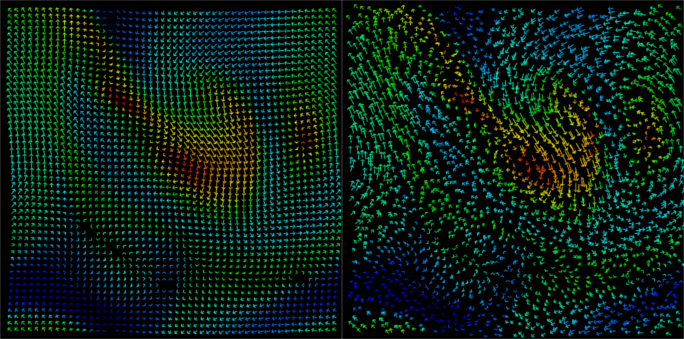
\includegraphics[width=\linewidth]{./content/pictures/jitter.png}
			  \caption{Uniform grid and jittered grid.}
			  \label{fig:jitter}
		\end{figure}


	\subsection{Glyph shapes}
		In addition to the lines that were already present, two other glyph shapes were added.
		We chose to implement arrows and triangles because these shapes can add extra insight in the data.
		The different shapes can be seen in Figure~\ref{fig:glyph_shapes}.
		\begin{figure}[htb]
		    \centering
		    \begin{subfigure}[htb]{.49\textwidth}
		        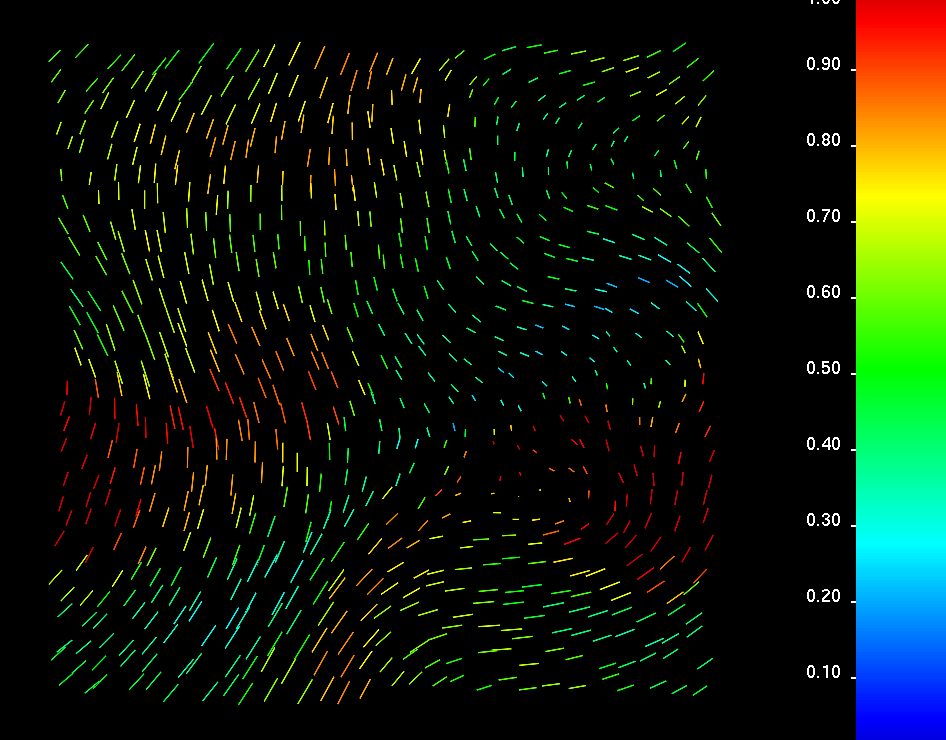
\includegraphics[width =\textwidth]{content/pictures/lines.png}
		        \caption{Lines}
		        \label{fig:lines}
		    \end{subfigure}
		    \begin{subfigure}[htb]{.49\textwidth}
		        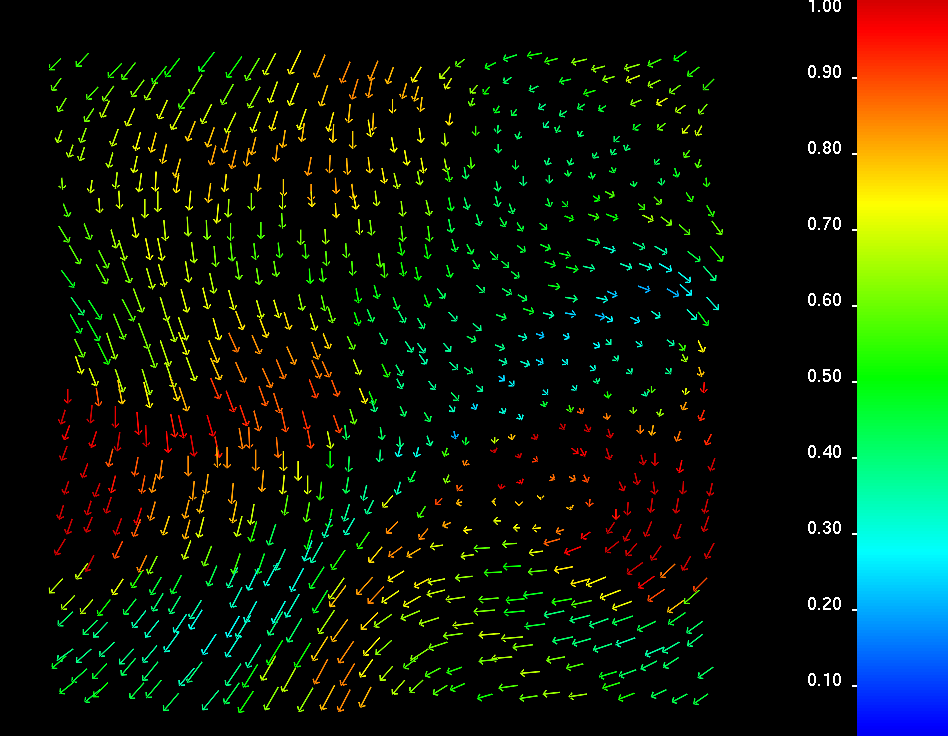
\includegraphics[width =\textwidth]{content/pictures/arrows.png}
		        \caption{Arrows}
		        \label{fig:arrows}
		    \end{subfigure}
		    \begin{subfigure}[htb]{.49\textwidth}
		        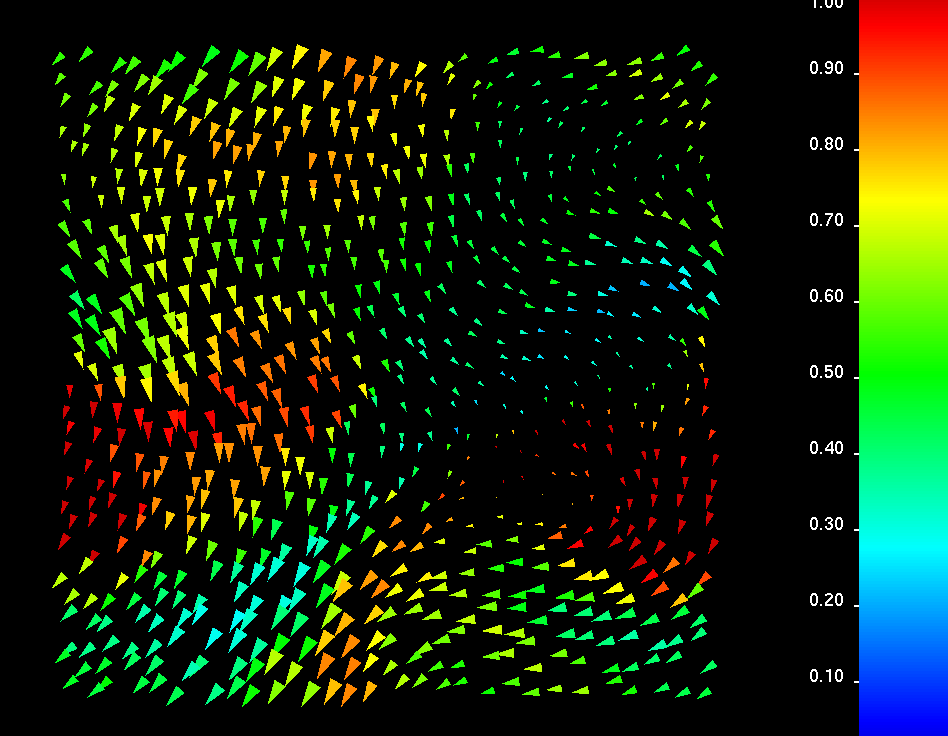
\includegraphics[width =\textwidth]{content/pictures/triangles.png}
		        \caption{Triangles}
		        \label{fig:triangles}
		    \end{subfigure}
		    \begin{subfigure}[htb]{.49\textwidth}
		        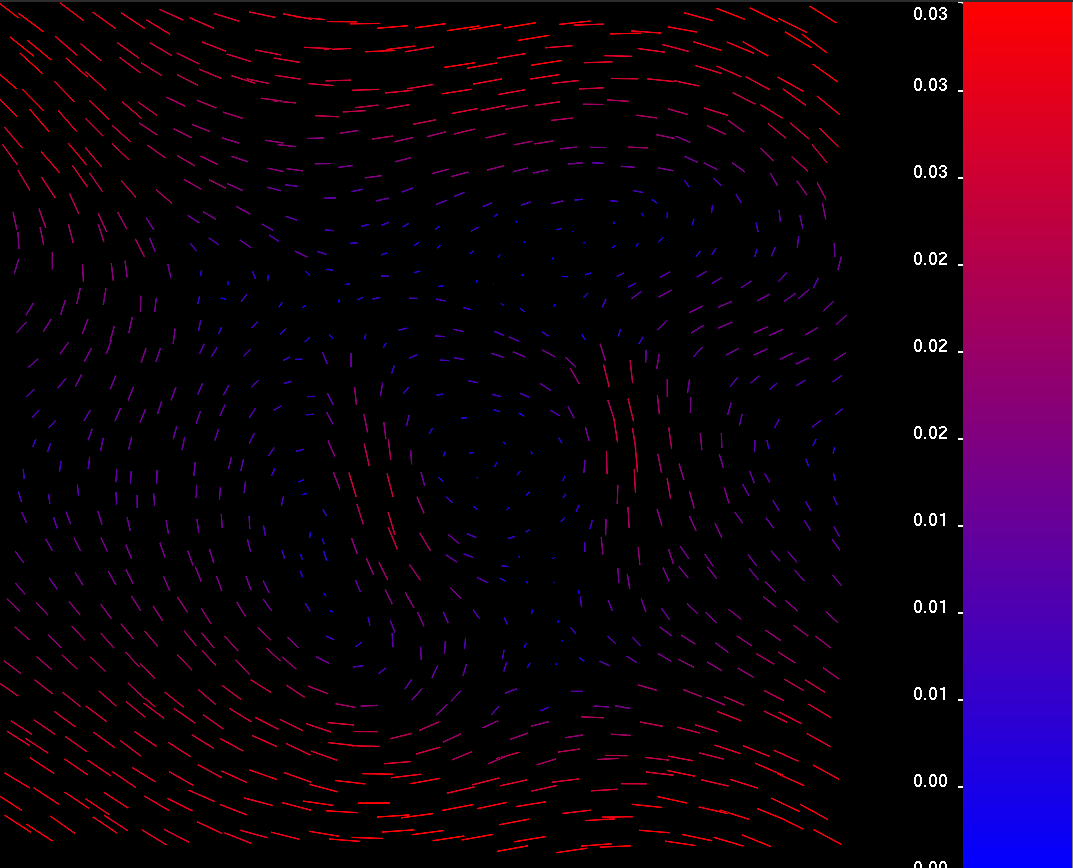
\includegraphics[width =\textwidth]{content/pictures/bipolar_glyphs.png}
		        \caption{Bipolar color map}
		        \label{fig:bipolar}
		    \end{subfigure}
		    \caption{Various glyph visualization techniques}
		    \label{fig:glyph_shapes}
		\end{figure}
		\subsubsection{Arrows}
			An arrow is created using the basic line that was already implemented, at the end of the line a `head' is constructed.
			The length of the arrow is the same as of the basic line. 
			Before drawing, the scene's coordinate system is translated and rotated to the appropriate orientation, using \texttt{glTranslatef} and \texttt{glRotatef}.
			Visualization using arrows on a jittered grid can be seen in figure~\ref{fig:arrows}.


		\subsubsection{Triangles}
			A triangle is created in such a way that the base has the smallest side of the triangle.
			This is done so it is easier to recognize in which direction the triangle is pointing to.
			The height of a triangle is the same as the length of a basic line.
			Visualization using triangles on a jittered grid can be seen in figure~\ref{fig:triangles}.
